\section{Iteration \#1 -- Evaluation Framework and Baselines}

TODO: outline of what this iteration is

\subsection{Data Generation}

TODO

\subsection{Evaluation Framework}

TODO: discuss design of this, what it does and WHY I decided to do it

TODO: what form an index structure takes -- i.e. its interface

\subsection{Baselines Implementations}

TODO: sequential scan and octree (describe remove() algorithm)

\subsection{Pyramid Tree}

TODO: how I got an implementation from a research fellow, etc. and modified it

TODO: added remove() and how I handled that

\subsection{Performance Analysis}

TODO: what I did for the performance analysis, what data I used, operation lists, etc.

TODO: show all the graphs, tables, etc.

\begin{figure}
	\centering
	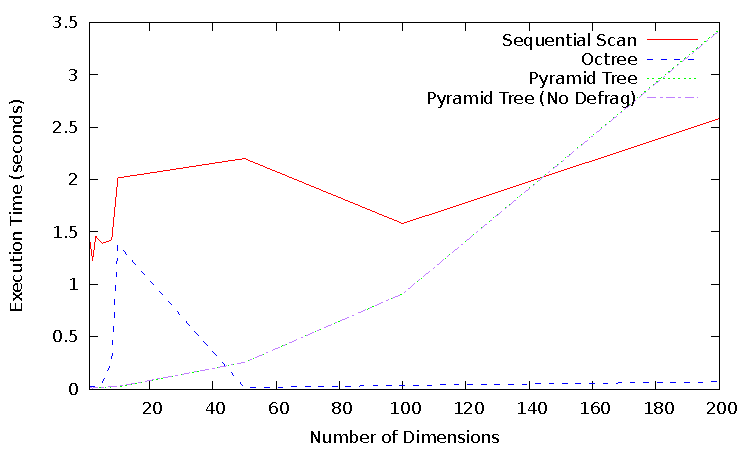
\includegraphics[scale=0.8]{../results/end_of_iteration1/all_insert_randuniform.pdf}
	\caption{\texttt{insert} Performance on Randomly Generated Uniformly Distributed Datasets}
	\label{fig:perf-1-allinsert}
\end{figure}

\begin{figure}
	\centering
	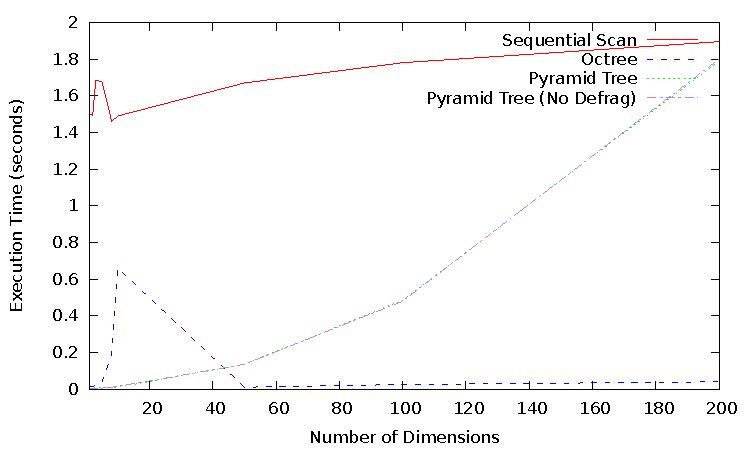
\includegraphics[scale=0.8]{../results/end_of_iteration1/all_pquery_randuniform.pdf}
	\caption{Point Query Performance on Randomly Generated Uniformly Distributed Datasets}
	\label{fig:perf-1-allpquery}
\end{figure}

\begin{figure}
	\centering
	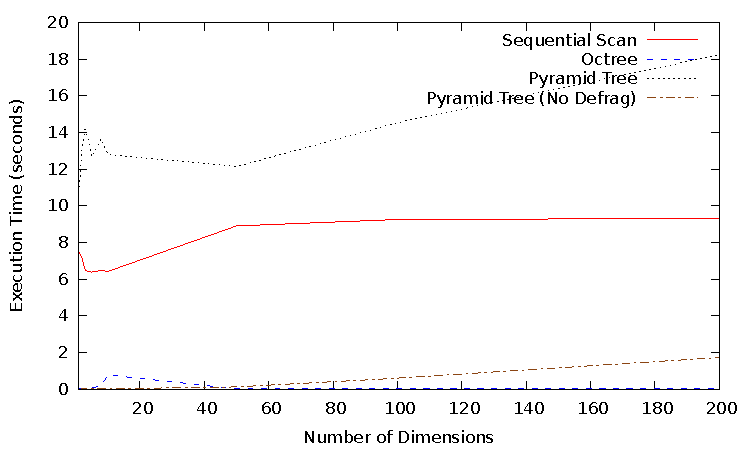
\includegraphics[scale=0.8]{../results/end_of_iteration1/all_delete_randuniform.pdf}
	\caption{\texttt{delete} Performance on Randomly Generated Uniformly Distributed Datasets}
	\label{fig:perf-1-alldelete}
\end{figure}

\subsection{Evaluation}

TODO: evaluate results in previous section

TODO state what was decided to do for next iteration (and why)
